
\section{Design}
\label{sec:design}

In this section we present the design of iProbe.
Additionally, we then explain some safety checks imposed by iProbe that ensure the correctness of our instrumentation scheme. 
Finally, we discuss extended iProbe modes, static binary rewriting and user written macros, which serve as alternatives to the default compiler-based scheme to insert instrumentation in the pre-processing stage of iProbe.

\begin{figure}[t]
  \begin{center}
    \includegraphics[width=0.75\textwidth]{iprobe/Images/coldpatch.eps}
    \caption{The Process of ColdPatching.}
    \label{fig:coldpatch}
  \end{center}
\end{figure}

The first phase of our instrumentation is an offline pre-processing stage to make the binaries ready for runtime instrumentation. We call this phase \emph{ColdPatching}. 
%meaning the static offline binary patch which is the opposite term to HotPatching to be explained next. 
The second phase is the an online \emph{HotPatching} stage which instruments the monitored program dynamically at runtime without shutting down and restarting the program. 
Next, we present the details of each phase.

%The current implementation of iProbe has been applied and tested in x86 32 bit and 64 bit systems on an centos 5.0, ubuntu, and red-hat system. Technically, however the implementation can be applied to any existing system by using compiler assistance and HotPatching.

\subsection{ColdPatching Phase}
\label{sec:coldpatch}


ColdPatching is a pre-processing phase which generates the place-holders for hooks to be replaced with the calls for instrumentation. 
This operation is performed offline before any execution by statically patching the binary file. 
This phase is composed of three internal steps that are demonstrated in Figure \ref{fig:coldpatch}. 

\begin{itemize}

\item Firstly, iProbe uses compiler techniques to insert instrumentation calls at the beginning and end of each function call. 
The instrumentation parameters, are decided on the basis of the design of the compiler pass. 
The current implementation by default passes callsite information and the base stack pointer as they can be used to inspect and form execution traces. 
Calls to the these instrumentation functions must be \emph{cdecl} calls so that stack correctness can be maintained, this is discussed in further detail in Section \ref{sec:safety}.

\item Secondly, iProbe parses the executable and replaces all instrumentation calls with a \texttt{NOP} instruction which is a no-operation or null instruction. 
This generates instructions in the binary which does no-operation, hence has a negligible overhead, and acts as an empty space for iProbe to be overwritten at run-time.

\item Thirdly, iProbe parses the binary and gathers meta-data regarding all the target instrumentation points into a \emph{probe-list}.
Optionally, iProbe can strip away all debug and symbolic information in the binary making it more secure and light-weight. 
The probe-list is securely transferred to the run-time interface of iProbe and used to probe the instrumentation points. 
Hence iProbe does not have to rely on debug information at run-time to HotPatch the binaries.

%In this way, iProbe differs from existing mechanisms as it does not rely on availability of debug information at run-time to HotPatch the binaries. 
\end{itemize}

%To allow for safe instrumentation using iProbe we need to prepare the target application binary. As described in section.\ref{sec:hotpatch}, to enable HotPatching there must be space allocated in the code segment of the binary to re-write instruction.Existing methodologies overwrite target instructions (eg. the starting instruction of the target instruction with a jump). However, this requires several additional steps to allocate memory and ensure sanity of the stack frames. 

%\indent To reduce complex binary transformations, we prepare the binary for run-time instrumentation before execution by using a coldpatch process.The steps of this process are shown in the state diagram shown in figure \ref{fig:state_rep}. 

%*** Longer version

%The first state is an instruction dump of an unmodified normal binary. As can be seen the initial instructions in each function after the call is made to the function are setting up the stack frame and then the main body. Hence, if any of these instructions are overwritten that would lead to potentially illegal execution states. Instead iProbe makes these binaries \textit{``HotPatch ready``} by introduce place holders in the binary which are used to create empty space. While a compiler transform or flag can be designed based on the target abstraction for instrumentation, for the sake of simplicity we use existing compiler flag options such as ``-finstrument-functions" \cite{gcc_codegen}. As shown in the figure.\ref{fig:state_rep} this flag option generates instrumentation calls at the entry and exit of every function. Just after the entry and before the exit of every function, calls are placed to \emph{\_cyg\_profile\_func\_enter} and \emph{\_cyg\_profile\_func\_exit}. 

%As step 2, we use a binary parser performs a linear scan to search and replace each of these function calls with a NOP instruction (state 3). The replacement needs to be done carefully to ensure that there is enough space to overwrite these NOP's with a call to our instrumentation function. Additionally we store the instruction pointer of each of these function calls, the function they belong to, and the symbolic name. By replacing each of these function calls with NOP instructions we introduce a ``zero-probe" effect in the binary, i.e. the modified binary executes the same as the original binary with negligible overhead.

%To counter address space layout randomization, we also capture offsets with the starting address of each binary. These offsets allow us to use the starting/load address as a anchor to do the instrumentation. In practice we found that the offsets compared to the load address of the executable in binary remain the same, even if load points may be changed.

%One of the advantages of preparing and using the ColdPatching approach is that natural abstractions in the build process can also be used to choose the scope of instrumentation. Instrumentation scope defines the libraries, files, functions, and modules that can be instrumented. iProbe can be used to pre-define the target files, libraries etc. to be compiled, this can be important in cases where the source code is only partially available to the user. This is common for many large scale projects which use proprietary 3rd party components.


\begin{figure*}[t]
  \begin{center}
    \includegraphics[width=0.99\textwidth]{iprobe/Images/state-diagram.eps}
    \caption{Native Binary, the State Transition of ColdPatching and
    HotPatching.}
    \label{fig:state_rep}
  \end{center}
\end{figure*}

\begin{figure}[t]
  \begin{center}
    \includegraphics[width=0.75\textwidth]{iprobe/Images/HotTracing.eps}
    \caption{HotPatching Workflow.}
    \label{fig:hottracing}
  \end{center}
\end{figure}

\subsection{HotPatching Phase}
\label{sec:hottracing}

Once the application binary has been statically patched (i.e., ColdPatched), instrumentation can be applied at runtime. 
Compared to existing trampoline approaches, \emph{iProbe does not overwrite any instructions in the original program, or allocate additional memory} when patching the binaries, and still ensures reliability. 
In order to have a \emph{low overhead}, and \emph{minimal intrusion} of the binary, iProbe avoids most of the complexities involved in HotPatching such as allocation of extra memory in the code segment or scanning code segments to find instrumentation targets in an offline stage. 
The process of HotPatching is as follows: \\
%
%The iProbe run-time hot-tracer is a separate process which monitors the target application. 

\begin{itemize}

\item Firstly, iProbe loads the relevant instrumentation functions in a shared library to the code-segment of the target process. 
This along with allocation of \texttt{NOP}s in the ColdPatching phase allows iProbe to avoid allocation of memory for instrumentation in the code segment. 

\item The probe-list generated in the ColdPatching phase is given to our run-time environment as a list of target probe points in the executable. 
iProbe can handle stripped binaries due to previous knowledge of the target instructions in the ColdPatching.

\item As shown in Figure \ref{fig:hottracing}, in our instrumentation stage, 
our HotPatcher attaches itself to the target process and issues an interrupt (time T1). 
It then performs a reliability check (see Section \ref{sec:safety}), 
and subsequently replaces the \texttt{NOP} instructions in each of the target functions, with a call to our instrumentation function. 
This is a key step which enables iProbe to avoid the complexity of traditional trampoline \cite{livepatch,katana} by not overwriting any logical instructions (non-\texttt{NOP}) in the original code. 
Since the place-holders (\texttt{NOP} instructions) are already available, iProbe can seamlessly patch these applications without changing the size or the runtime footprint of the process. 
Once the calls have been added iProbe releases the interrupt and let normal execution proceed (time T2).

\item At the un-instrumentation stage the same process is repeated, with the exception that the target functions are again replaced with a \texttt{NOP} instruction. 
The period between time T2 and time T3 is our monitoring period, wherein all events are logged to a user-space shared memory logger.

\end{itemize}

\noindent \textbf{State Transition Flow}: \quad Figure \ref{fig:state_rep} demonstrates the operational flow of iProbe in the example to instrument the entry and exit of the \texttt{func\_foo} function. 
The left most figure represents the instructions of a native binary. 
As an example, it shows three instructions (i.e., push, pop, inc) in the prolog and one instruction (i.e., pop) in the epilog of the function \texttt{func\_foo}. 
The next figure shows the layout of this binary when it is compiled with the instrumentation option. 
As shown in the figure, two function calls, \texttt{foo\_begin} and \texttt{foo\_end} are automatically inserted by the compiler at the start and end of the function respectively. 
iProbe exploits these two newly introduced instructions as the place-holders for HotPatching. 
The ColdPatching process overwrites two call instructions with \texttt{NOP}s. 
At runtime, the instrumentation of \texttt{func\_foo} is initiated by HotPatching those instructions with the call instructions to the instrumentation functions: \texttt{begin\_instrument} and \texttt{end\_instrument}. 
This is illustrated in the right most figure in Figure \ref{fig:state_rep}.

\noindent \textbf{Logging Functions and Monitoring Dispatchers} : \quad
%
The calls from the target function to the instrumentation function are generally defined in the coldpatch stage by the compiler. 
However, iProbe also provides monitoring dispatchers which are common instrumentation functions that are shared by target functions. 
Our default instrumentation passes the call site information, and the function address of the target function as parameters to the dispatchers. 
Each monitoring event can be differentiated by these dispatchers using a quick hashing mechanism representing the source of each dispatch.
This allows iProbe to uniquely define instrumentation for each function at run-time, and identify its call sites.

\subsection{Safety Checks for iProbe}
\label{sec:safety}

Safety and reliability of the instrumentation technique is a big concern for most run-time instrumentation techniques.
One of the key advantages of iProbe is that because of its hybrid design reliability and correctness issues are handled in a better way inherently.
In this section we discuss how our HotPatch can achieve such properties in details.
%As explained earlier iProbe operates in 3 different modes,(1) compiler-assisted (2) User-macro based, and (3) static binary rewriting.

\indent \textbf{HotPatch check against Illegal instructions}: \quad
Unlike previous techniques iProbe relies on compiler correctness to ensure safety and reliability in its binary mode.
%The resulting instrumented binary in ColdPatch is not only safe but optimized.
To ensure correctness in our ColdPatching phase, we convert call instructions to instrumentation functions with \texttt{NOP} instruction. 
This does not in any way effect the correctness of the binary, except that instrumentation calls are not made. 
To ensure run-time correctness, iProbe uses a safety check when it interrupts the application while HotPatching. 
Our safety check pass ensures that the program counters of all threads belonging to the target applications do not point to the region of code that is being overwritten (i.e. \texttt{NOP} instructions are not overwritten while they are being executed.
This check is similar to those from traditional Ptrace\cite{ptrace} driven debuggers etc \cite{kaho,livepatch,pannus}. 
Here we use the Ptrace \texttt{GETREGS()} call to inspect the program counter, and if it is currently pointing to the target \texttt{NOP} instructions, we allow the execution to move forward before applying the HotPatch. 
Unlike existing trampoline oriented mechanisms iProbe has a small \texttt{NOP} code segments equal to the length of a single call instruction that it overwrites with instrumentation calls, this means that the check can be performed in a fast and efficient manner. 
It is also important to have this check for all threads which share the code-segment, hence the checking must be able to access the process memory map information, and interrupt all the relevant threads.

\indent \textbf{Safe parameter passing to maintain stack consistency}: \quad
An important aspect for instrumentation is the information passed along to the instrumentation function via the parameter values. 
Since the instrumentation calls are defined by the compiler driven instrumentation, the mechanism in which the parameters passed are decided based on the calling convention used by the compiler. \\
Calling conventions can be broadly classified in two types: caller clean-up based, and callee clean-up based. 
In the former the caller is responsible to pop the parameters passed to function, and hence all parameter related stack operations are performed before and after the call instruction inside the code segment of the caller.
In the later however, the callee is responsible to pop the parameters passed to it.
Since parameters are generally passed using the stack it is important to remove them properly to mantain stack consistency. 

To ensure this iProbe enforces that all calls that are made by the static compiler instrumentation must be \emph{cdecl}~\cite{cdecl} calls where the caller performs the cleanup as compared to \emph{std} calls, where the callee performs it. 
%\emph{cdecl} calls push instrumentation parameters before the call, and stack cleanup is also performed by caller function. 
%On the other hand in \emph{std} call convention the stack cleanup is performed by the callee. 
%For simplicity sake, iProbe uses only \emph{cdecl} calls and allows the push and pop operations performed by the caller. 
As the stack cleanup is automatically performed, it maintains stack consistency, and there is a negligible impact in performance due to the redundant stack operations. 
Alternatively for \emph{std} call convention, push instructions could also be converted to \texttt{NOP}s and HotPatched at run-time, we do not do so as a design choice. 

\indent \textbf{Address Space Layout Randomization}: \quad
Another issue that iProbe addresses is ASLR (address space layout randomization), a security measure used in most environments which randomizes the loading address of executables and shared libraries. 
However, since iProbe assumes the full access to the target system, the load addresses are easily available. 
HotPatcher uses the process id of the target to find all load addresses of each binary/shared library and uses them as base offsets to generate correct instruction pointer addresses. 


%\textbf{Developer Driven Macros}
% The developer driven Macros

%\textbf{Static Binary Rewriter}


\subsection{Extended iProbe Mode}
\label{sec:advanced}

%Since the default mode of iProbe is compiler driven using instrumentation flags.
As iProbe ColdPatching requires compiler assistance, it is unable to operate on pre-packaged binary applications.
Additionally, compiler flags generally have limited instrumentation flexibility as they generally operate on a programming language abstraction(eg. function calls, loops etc.).
To provide further flexibility, iProbe provides a couple of extended options for ColdPatching of the application

\subsubsection{Static Binary Rewriting Mode} 
 In this mode we use a static binary rewriter to insert instrumentation in a pre-packaged binary. 
Once all functions are instrumented, we use a ColdPatching script to capture all call sites to the instrumentation functions and convert them to \texttt{NOP} instruction.
While this mode allows us to directly operate on binaries, a downside is that our current static binary instrumentation technique also uses mini-trampoline mechanisms. 
As explained in Section \ref{sec:trampoline} static binary rewriters use trampoline based mechanisms which induces minimum two jumps.
In the ColdPatch phase, we convert calls to the instrumentation function to \texttt{NOP}s, however the jmp operations to the trampoline function, and simulation of the overwritten instructions still remain.
The downside of this approach has a small overhead even when instrumentation is turned off.
However, in comparison to pure dynamic instrumentation approach it reduces the time spent in HotPatching.
This is especially important if the number of instrumentation targets is high, and the target binary is large, as it will increase the time taken in analyzing the binaries. 
Additionally, if compiler options cannot be changed for certain sections of the program (plugins/3rd party binaries), iProbe can still be applied using this extended feature.

Our current implementation uses the dyninst \cite{dyninst} and cobi \cite{cobi} to do static instrumentation. 
This allows us to provide the user a configuration file and template which can be used to specify the level of instrumentation (e.g., all entry and exit points for instrumentation), or names of specific target functions, and the instrumentation to be applied to them.
Subsequently in ColdPatch we generate our meta-data list, and use it to HotPatch and apply instrumentation at run-time.

\subsubsection{Developer Driven Macros}
% To provide further flexibility, iProbe provides a developer driven mode using user placed macros as required. 
%For example, compiler based instrumentation is able to insert entry and exit of each function(or other programming abstractions), however at times it may be required to inspect a certain line of code or instruction.
Compiler assisted instrumentation may not provide complete flexibility (usually works on abstractions, such as enter/exit of functions), hence for further flexibility, iProbe provides the user with a header file with calls to macros which can be used to add probe points in the binary.
A call to this macro can be placed as required by the developer. 
The symbol name of the macro is then used in the ColdPatch stage to capture these macros as probe points, and convert them to \texttt{NOP}s.
Since the macros are predefined, they can be safely inserted and interpreted by ColdPatcher.
The HotPatching mechanism is very much the same, using the probe list generated by ColdPatch.

%iProbe hot-tracing completely operates in the user-space hence there is no overhead of context-switches because of software/kernel trap mechanisms \cite{dtrace,sytemtap,lttng}. In the evaluation section, we compare the performance of iProbe with current state-of-the-art approaches.

%Once the application is \textit{"coldpatched"}, instrumentation can be applied at run-time. Figure.\ref{fig:hottracing}, shows a step wise diagram of a normal usage case scenario for iProbe. As mentioned earlier in section.\ref{sec:hotpatch} HotPatching needs to load the code segment and activate or deactivate instrumentation as required by the user.Before executing the program all instrumentation code is preloaded in the execution environment. This ensures that the instrumentation library is a part of the code segment of the target application.

%The hot-tracer itself is an interactive GUI interface, that assists the user in easy Hot-Tracing. As a first step, the user needs to find the process id of the target process, this can be done by using various utility programs such as ps, ptrace etc. The user then needs to provide the list of instrumentable points which are generated in ColdPatch phase This is the entire list of potential instrumentation points that can be enabled by the user. 

%Once provided to the hot-tracer, iProbe then provides the user various function and resource level abstractions to do the instrumentation. The symbolic information used in this step is already read from symbolic information read from the binary at the ColdPatching time. The user can choose one or many functions, files or libraries to be the target instrumentation set. This file/component/library to target function relationship\footnotetext[1]{file/component/library to target function relationship may not be available at run-time depending on the amount of debugging information available in the binary, symbolic information may be turned off for production systems} is something which gives a good insight when doing the debugging. 
% **add to the footnote information about binary obfuscation

%Function are shown in the following format:
%\begin{verbatim}
%<Symbol Name, Entry\Exit Point,Source File>
%\end{verbatim}

%The instrumentation set is taken by the hot-tracer(step 2 in figure \ref{fig:hottracing}) and the process is instrumented. Our current implementation uses ptrace \cite{ptrace}, a Linux utility tool to search and overwrite instrumentation 


% RHEE: I feel dual space seems ackward to be presented here.
% We emphasized the entire user level tracing. But here kernel level
% tracing comes into the play.

% \subsection{Dual Space Architecture}
% \label{dualspace}
% 
%  As described in section.\ref{sec:related_work}, most existing systems have a single recording mechanism \cite{dtrace,systemtap,fay,lttng} ; Hence, in a live recording scenario for any user-space event, these tools have a context-switch to kernel space either to introduce instrumentation via kernel techniques (viz. trap mechanisms used in DTrace and SystemTap \cite{dtrace,systemtap}), or because the recording mechanism is in the kernel \cite{fay}. This induces an unnecessary overhead because of the context-switch.To avoid these context-switches while at the same time obtaining a unified kernel and user-space trace, iProbe uses a novel dual-space architecture.  
% 
% \begin{figure}[htb]
%   \begin{center}
%   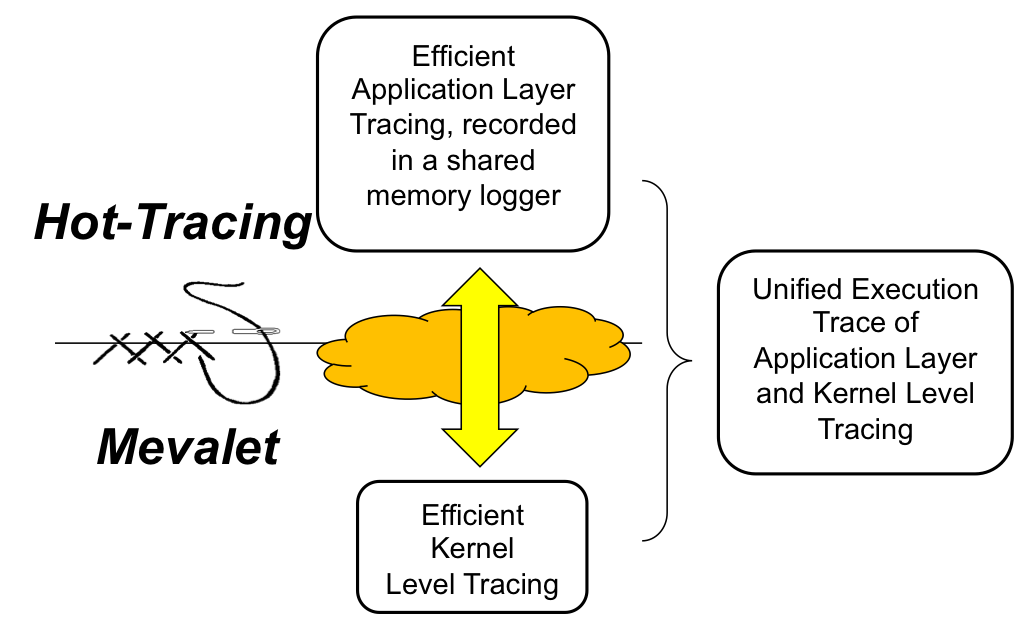
\includegraphics[width=0.5\textwidth]{Images/Dual-Space.eps}
%   \caption{Dual-Space Mechanism}
%   \label{fig:dualspace}
%  \end{center}
% \end{figure}
% 
% 
% iProbe records user-space events in a shared memory user-space logger, simultaneously kernel events are recorded in kernel space using a separate logger called Mevalet \footnote{Mevalet is a proprietary light-weight kernel event logger used in several production environments}. At the end of the recording interval, the log files of both user-space and kernel-space are "stitched" together to get a single execution trace. This avoids any unnecessary context-switches at the production run-time.
% 
% iProbe uses thread local storage to log all events to avoid potential race conditions. To ensure that causal relationships\footnote{theoretically misalignment is possible however to keep a low overhead we have kept a lock-free mechanism} are maintained between kernel traces and user-space traces. iProbe issues dummy system calls which are caught in the kernel log, these are then used along with the time stamps to align both traces into a single unified view.
% 
% When stitching the traces together we use a regression mechanism to align both the traces together.

%iProbe has been built on top of a production level kernel tracer, Mevalet \cite{mevalet}. The key idea behind dual-space architecture is simple, iProbe records user-space events in a shared memory user-space logger. While Kernel Events are recorded using Mevalet a proprietary kernel tracing tool (similar to SystemTap\cite{systemtap}), with a buffered kernel recorder. At the end of the recording interval, the log files of both user-space and kernel-space are stitched together to get a single execution trace. This avoids any unnecessary context-switches at the production run-time.

%iProbe uses rdtsc counters\cite{rdtsc} to measure time along with with the event log, to get a causal order of the events recorded. To ensure that race-conditions do not occur, shared memory logger buffers are maintained by using thread local storage\cite{tls} of every thread. Since events are recorded in a per-thread basis (it is not possible to have race conditions etc.) we assume causal consistency in the event log.  

%Lastly at the end of the recording period iProbe \textbf{stitches} kernel and user-space traces. To ensure that causal relationships are maintained between kernel traces and user-space traces; iProbe issues dummy system calls which are caught as events in the user-space, which are at the same time captured by the kernel space recorders.  At the initiation of every process 4 such system calls are triggered and captured at both user-space and kernel logs. When stitching the traces together we use a regression mechanism to align both the traces together.

% Add how we use regression and anchors to stitch the two together


%\subsection{Dispatcher: Function Selection}

%As described in the previous section, once a function is selected for instrumentation a call is made to the instrumentation by HotPatching. However, there can be potentially a large number of functions belonging to the target binary 
